%% Standalone supplementary material: second implementation (FEniCSx) of cavityFlexibleBottom.
%% DRAFT. Build (from this directory):  latexmk -pdf supplement_fenicsx_cavityflexiblebottom.tex
%% It does not read article.aux (no cross-references to the main article), so it builds on its own.
%% Bibliography keys Baratta2023 (DOLFINx) is added to bibliography.bib by the open draft PR #69; PETSc, MUMPS:1, MUMPS:2, Tukovic2018 are already in bibliography.bib.
%% Data, scripts and provenance: paper-data/fenicsx_cavityflexiblebottom/ (README.md there).
\documentclass[sn-mathphys,Numbered]{sn-jnl}
\usepackage{graphicx}
\usepackage{amsmath,amssymb,amsfonts,bm}
\usepackage{xcolor}
\usepackage{soul}
\usepackage{manyfoot}
\usepackage{booktabs}
\usepackage{siunitx}
\usepackage{float}
\usepackage[utf8]{inputenc}
\usepackage[onehalfspacing]{setspace}
\usepackage[section]{placeins}
\usepackage{geometry}
\geometry{a4paper,textwidth=15cm,textheight=24cm}
\setlength{\parskip}{\baselineskip}

%% S-prefixed numbering
\renewcommand{\thesection}{S\arabic{section}}
\renewcommand{\thefigure}{S\arabic{figure}}
\renewcommand{\thetable}{S\arabic{table}}
\renewcommand{\theequation}{S\arabic{equation}}

\newcommand{\todo}[1]{\par\noindent\textcolor{red}{\rule{\linewidth}{0.8pt}}\par\nopagebreak
	\noindent{\small\color{red!70!black}\textbf{AUTHOR NOTE:} #1\par}\nopagebreak
	\noindent\textcolor{red}{\rule{\linewidth}{0.8pt}}\par}
\newcommand{\legacy}{\textcolor{red!70!black}{legacy moving-wall BC; reruns after solids4foam PR~\#671 pending}}
\newcommand{\legbc}{\textcolor{red!70!black}{(legacy BC)}}

\begin{document}

\title[Supplementary material: FEniCSx cavityFlexibleBottom]{Supplementary material: a second implementation of cavityFlexibleBottom (FEniCSx), by the same group and tooling lineage}

\author*[1]{\fnm{Author} \sur{Placeholder}}\email{corresponding.author@example.org}
\author[1]{\fnm{Author} \sur{Placeholder 2}}

\affil[1]{\orgdiv{School of Mechanical and Materials Engineering}, \orgname{University College Dublin}, \orgaddress{\country{Ireland}}}

\maketitle

\todo{DRAFT, supplementary to the cavityFlexibleBottom material (PRs \#12, \#14, \#18, \#20, \#22, \#23, \#27, \#67). Author list, CRediT and the AI-use paragraph are placeholders for the authors to agree. Numbers come from the CSV files in \texttt{paper-data/fenicsx\_cavityflexiblebottom/}; hashes, commits, job identifiers, retained failed runs and the audit lineage are in its README. \textbf{Every solids4foam value below was computed with the \legacy{}.} Decision requested from the reviewers: whether a second implementation of the cavity belongs in the supplement at all. No manuscript text is changed.}

\section{Scope and disclosure}\label{sec:cv_scope}
The cavityFlexibleBottom references in the suite are four solids4foam, Tukovi\'c, ANSYS and COMSOL sequences; the solids4foam partitioned and quasi-monolithic sequences have Richardson limits of $u_y(A)\approx-0.2407\,\mathrm{m}$ and $F_y\approx-5.26\,\mathrm{N/m}$ \legbc.
This supplement adds a \emph{second implementation by the same group and tooling lineage}: monolithic finite elements on conforming triangles (FEniCSx), solving the St~Venant--Kirchhoff (StVK) plane-strain model with the exact interface traction, on four consistently refined meshes.
It is not an independent verification.
The problem definition, the mesh block structure (refined from the tutorial's), the monitoring point and the convergence routine are shared with the reference runs; the code was written, run and audited by AI agents of one model family for the same group.
One audit was made by a further agent of that family (internal, not a human or external review; verdict QUALIFIED); its required wording restrictions are applied here.
No external review has taken place.
``Preregistered below means written before the runs, with self-asserted timestamps; the two files are in the package (\texttt{preregistration/}) and the hashes of the originals cannot be checked from it.
The milestone concerns the exact model only.

\section{Model, solver and meshes}\label{sec:cv_model}
\paragraph{Problem.}
The tutorial case: channel $[0,14]\times[1,2]\,\mathrm{m}$ over a cavity $[2,6]\times[0,1]\,\mathrm{m}$ with radius-$0.25\,\mathrm{m}$ rounded upper corners, closed at the bottom by a plate $[2,6]\times[-0.4,0]\,\mathrm{m}$ clamped on both end faces, underside free, StVK, plane strain, $E=500\,\mathrm{Pa}$, $\nu=0.4$, $\rho_s=1000$; fluid $\rho_f=1$, $\nu_f=0.01$ ($\mathrm{Re}=100$), parabolic inlet of mean $1\,\mathrm{m/s}$, outlet $p=0$.
Point $A=(4,0)$ is mid-span of the wetted top surface.
\paragraph{Solver.}
DOLFINx~\citep{Baratta2023} with PETSc SNES~\citep{PETSc} and a MUMPS direct solver~\citep{MUMPS:1,MUMPS:2}; monolithic ALE, unknowns $(\bm u\,P_2,\ p\,P_1,\ \bm d\,P_2)$ on one mesh, total-Lagrangian StVK plate, harmonic fluid mesh motion with inverse-volume stiffness, backward Euler in pseudo-time ($\Delta t=10\,\mathrm{s}$, inlet ramp $\tfrac12[1-\cos(\pi t/20)]$ for $t<20\,\mathrm{s}$, stop when the relative rate of $u_y(A)$ and of $F_y$ stays below $10^{-6}\,\mathrm{s^{-1}}$ for three steps after $60\,\mathrm{s}$).
\paragraph{Interface (M1).}
The fluid and plate share the test function on the interface, so the plate receives $\bm\sigma_f\bm a$ per reference area with $\bm a=J\bm F^{-T}\bm N$ (exact Nanson), i.e.\ the fluid traction acting on the \emph{current} area $\mathrm d s=|\bm a|\,\mathrm dS_0$. This is called M1.
\paragraph{Differences from the tutorial (not isolated).}
monolithic against partitioned coupling; $P_2/P_1$ triangles (twice the tutorial cell count at equal $\Delta x$, exact circular arcs) against finite volumes; harmonic inverse-volume against inverse-distance mesh motion; a natural do-nothing outlet against fixed $p$ with zero-gradient $\bm u$ (equal to $10^{-6}$ in $F_y$ on a rigid floor, Section~\ref{sec:cv_pre}, not quantified in the coupled problem); a cosine inlet ramp against an impulsive start (the steady state does not depend on it); the solids4foam solid carries damping and a stabilisation term that vanish with refinement.
\paragraph{Meshes.}
$\Delta x=0.1$, $0.05$, $0.025$, $0.0125$ (L1--L4): $3376$ to $216064$ fluid and $320$ to $20480$ plate triangles, $0.03$ to $2.0$ million unknowns, four to thirty-two cells through the plate thickness; fluid area $5\times10^{-8}$ (L1) to $2\times10^{-11}$ (L4) from the exact value. Meshes are regenerated from the committed geometry files (gmsh 4.14.0) and hash-checked (README).

\section{Spatial convergence}\label{sec:cv_spatial}
All four levels met the registered steady criterion and the validity gates (Section~\ref{sec:cv_gates}).
Orders and limits use the routine of the main article (monotone, $0.5\le p\le3$, $F_s=1.25$) on triples of levels; the steady drift at stop is $4.7\times10^{-7}\,\mathrm{s^{-1}}$ ($u_y$) and $2.5\times10^{-8}\,\mathrm{s^{-1}}$ ($F_y$).
\begin{table}[htbp]
\centering
\caption{FEniCSx M1, steady values. $F_y$: direct Nanson integral of the fluid traction on the plate (viscous part $0.03\,\%$); the weak force including the clamp-corner dofs agrees to $<2\times10^{-5}$. \texttt{data/coupled\_levels.csv}.}\label{tab:cv_levels}
\small
\begin{tabular}{@{}lrrrrrrr@{}}
\toprule
Level & $\Delta x$ (m) & $u_y(A)$ (m) & $u_x(A)$ (m) & $F_y$ (N/m) & $F_x$ (N/m) & Newton its & CPU-h \\
\midrule
L1 & 0.1 & $-0.2390188$ & $9.5207\!\times\!10^{-5}$ & $-5.259171$ & $-0.016688$ & 99 & 0.026 \\
L2 & 0.05 & $-0.2399405$ & $9.6087\!\times\!10^{-5}$ & $-5.257991$ & $-0.016652$ & 106 & 0.118 \\
L3 & 0.025 & $-0.2402963$ & $9.6477\!\times\!10^{-5}$ & $-5.257843$ & $-0.016628$ & 109 & 0.827 \\
L4 & 0.0125 & $-0.2404424$ & $9.6676\!\times\!10^{-5}$ & $-5.257811$ & $-0.016618$ & 110 & 5.853 \\
\bottomrule
\end{tabular}
\end{table}
\begin{table}[htbp]
\centering
\caption{Observed order $p$, Richardson limit and GCI for the two triples. \texttt{data/coupled\_orders.csv}.}\label{tab:cv_orders}
\small
\begin{tabular}{@{}lrrrrrr@{}}
\toprule
 & \multicolumn{3}{c}{L2--L4} & \multicolumn{3}{c}{L1--L3} \\
\cmidrule(r){2-4}\cmidrule(l){5-7}
Quantity & $p$ & limit & GCI (\%) & $p$ & limit & GCI (\%) \\
\midrule
$u_y(A)$ (m) & 1.28 & $-0.240544$ & 0.053 & 1.37 & $-0.240520$ & 0.116 \\
$F_y$ (N/m) & 2.18 & $-5.257801$ & $2\times10^{-4}$ & 3.0002 & \multicolumn{2}{c}{not accepted} \\
$u_x(A)$ (m) & 0.97 & $9.688\!\times\!10^{-5}$ & 0.27 & 1.18 & $9.679\!\times\!10^{-5}$ & 0.40 \\
\bottomrule
\end{tabular}
\end{table}
\paragraph{What the orders support.}
The $u_y$ order is about $1.3$ and \emph{pre-asymptotic}: it falls from $1.37$ to $1.28$ with refinement, so the asymptotic range is not demonstrated, and no second-order statement is made for $u_y$. If the true order were anywhere in $[1,2]$ the extrapolated limit would move by $-0.018\,\%$ to $+0.022\,\%$ (signed value: negative means larger $|u_y|$; \texttt{data/coupled\_uy\_limit\_vs\_order.csv}), the same size as the quoted GCI; the limit is therefore known to about $\pm0.02$--$0.05\,\%$ and not better.
\paragraph{Clamp-corner hypothesis (consistent, not proved).}
The plate-only Q2 ladder extended to 32 elements through the thickness gives orders $1.394$ ($4,8,16$) and $1.298$ ($8,16,32$), limit $-0.241358\,\mathrm m$ (GCI $0.03\,\%$) for a uniform load, and $1.392$, $1.299$, limit $-0.239854\,\mathrm m$ for the recorded follower load (\texttt{data/plate\_only\_q2\_nt32\_orders.csv}); Q3 gives the same limits to $10^{-6}$ and similar orders ($1.29$) at any degree. The linearised plane-strain problem of a $90^\circ$ wedge clamped on one edge and free on the other ($\nu=0.4$) has the leading Williams exponent $\lambda=0.6499$, so $2\lambda=1.2998$ (a root of $1+\kappa^2+2\kappa\cos\pi\lambda=4\lambda^2$, $\kappa=3-4\nu$; \texttt{data/williams\_exponent.csv}). The observed orders drift towards it. This is numerical evidence \emph{consistent with} corner-controlled convergence, not a proof: the derivation covers only the linearised wedge eigenvalue, not the finite-strain StVK problem, and not the step from the exponent to the point-value order at $A$. By the assessment of the work (not recomputed here), at least $94\,\%$ of the coupled $u_y$ increments between levels are structural rather than fluid-borne. A preregistered discriminating experiment (graded plate meshes; confirm if the graded order is $\ge2.5$, reject if $\le1.6$) produced \textbf{no result}: every graded case with $\ge8$ elements through the thickness diverged in Newton (aspect ratios up to $5\times10^{3}$), also with load continuation, so the hypothesis is neither confirmed nor rejected (recorded as NOT TESTED; $0.201$ CPU-h; \texttt{data/graded\_mesh\_attempts.csv}). The solids4foam sequences give an order of about $2.0$ for the same quantity \legbc{} (strict partitioned $2.03$, PR~\#14); the same clamps exist in the finite-volume runs, so the order difference is not explained by this work.
$L_4$ differs from the $u_y$ limit by $0.042\,\%$ and $L_3$ from $L_4$ by $0.061\,\%$.
The $F_y$ order $2.2$ rests on one accepted triple (L1--L3 gives $p=3.0002$, outside the accepted range, and is not extrapolated); $L_4$ differs from its limit by $1.7\times10^{-4}\,\%$.
The support-reaction ``order'' of $0.97$ sometimes quoted for these data is an artefact and is not reported: the reported reactions exclude the clamp-corner dofs, and the deficit $R_{l,y}+R_{r,y}+F_y$ ($-0.04745$, $-0.02393$, $-0.01212$, $-0.00615$) halves with every level, i.e.\ it is proportional to $\Delta x$ (\texttt{data/reaction\_deficit.csv}).

\paragraph{Pseudo-time stop error, time step, solver tolerance.}
At the stop the $u_y$ increments are still ringing (L2, last eight steps: $-8.0\times10^{-5}$, $-4.8\times10^{-5}$, $-6.8\times10^{-6}$, $+9.3\times10^{-6}$, $+7.7\times10^{-6}$, $+2.1\times10^{-6}$, $-8.5\times10^{-7}$, $-1.1\times10^{-6}\,\mathrm m$): the undamped plate is brought to rest by the dissipation of backward Euler only, and the criterion means ``steady to about $5\times10^{-6}$ relative'', not machine-steady. The remaining error is about $10^{-6}\,\mathrm m$, equal on all levels to $2\,\%$ (it cancels in level differences) and well below the L3--L4 difference ($1.5\times10^{-4}\,\mathrm m$).
Halving $\Delta t$ on L2 changes $u_y$ by $1.9\times10^{-6}$ and $F_y$ by $6\times10^{-8}$ (relative; the fixed point of backward Euler does not depend on $\Delta t$); on L1, $\Delta t=2.5$ gives $1.1\times10^{-5}$; $\Delta t=20$ diverges at the first step (kept). A tighter Newton tolerance on L1 changes $u_y$ by $2\times10^{-14}$. Rigid-wall limit (plate stiffened $10^5\times$): $F_y$ equals the frozen fixed-wall load to $1.6\times10^{-7}$; at $10^7\times$ it agrees to $1.6\times10^{-9}$ for 14 steps and Newton then fails (retained, attributed to the $10^{9}$ stiffness ratio, not shown).
\begin{figure}[htbp]
\centering
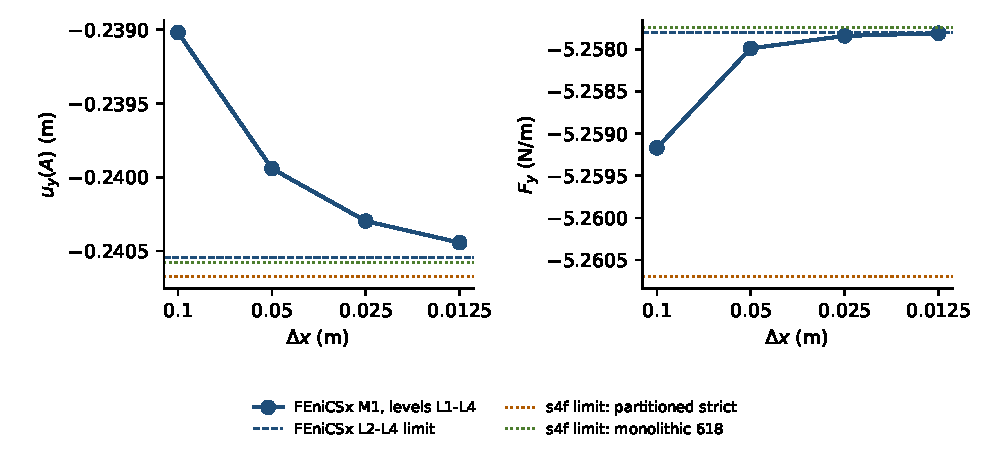
\includegraphics[width=0.85\textwidth]{paper-data/fenicsx_cavityflexiblebottom/figures/fenicsx_cavity_spatial}
\caption{FEniCSx M1 steady $u_y(A)$ and $F_y$ against $\Delta x$, with the FEniCSx L2--L4 limit and two solids4foam limits (\legbc).}\label{fig:cv_spatial}
\end{figure}

\section{Consistency gates are not physical validation}\label{sec:cv_gates}
On every level: interface-velocity error $\le1.6\times10^{-17}$; weak fluid power equals plate power to $\le8.2\times10^{-12}$; relative balance residual (supports $+$ weak fluid force $-$ inertia) $\le3.2\times10^{-12}$; minimum fluid Jacobian $0.963$--$0.964$, minimum plate Jacobian $0.91$ (L1) to $0.77$ (L4); no inversion.
\textbf{These are algebraic identities of the monolithic form} (shared test function): they certify that the implementation is internally consistent and not that the constitutive law, the geometry or the coupling measure is physically right; a wrong StVK constant would pass them. The physical checks are the preflight tests (Section~\ref{sec:cv_pre}) and the comparison with the solids4foam limits (Section~\ref{sec:cv_ref}).
Mass: the backward-Euler discrete-GCL defect equals its closed form $-\Delta t^{-1}\!\int J_1\det(\bm F_1^{-1}\nabla(\bm d_1-\bm d_0))$ to $5\times10^{-13}$ and is a property of the large first pseudo-time increments. Its \emph{absolute} peak is $4.15\times10^{-4}$ to $4.16\times10^{-4}$ (step~2, all levels), and $7.8\times10^{-4}$ only when normalised by the instantaneous inflow, which is $0.5$ at step~1 because of the inlet ramp. At the steady state it is $\le4.4\times10^{-13}$.
\paragraph{Reproduction.}
A further agent re-ran L1 from a fresh archive of the recorded commit (job 16673, 2 ranks): 21 steps, identical Newton counts, maximum relative difference to the original $6.6\times10^{-13}$; a 4-rank run agrees to $9.7\times10^{-13}$. This reproduces the pipeline for L1 only; L2--L4 were not rerun and it is not an independent implementation.

\section{Preflight: plate only and fluid only}\label{sec:cv_pre}
Before coupling, the two halves were run separately (preregistered gates, all passed; \texttt{data/plate\_only\_*.csv}, \texttt{fluid\_only\_*.csv}).
\paragraph{Plate only (StVK, Q2/Q3, $2$ to $16$ elements through the thickness).}
Under the recorded solids4foam level-2 pressure \legbc{} applied as a follower load (Cauchy pressure on the deformed surface), $u_y(A)=-0.23979\,\mathrm m$ at the finest level; order $1.29$--$1.39$, GCI $0.03$--$0.07\,\%$. Treating the same pressure as a reference-configuration load overstates $u_y$ by $3.05\,\%$ (recorded face-force vectors held fixed: $+0.11\,\%$): this is the measure ambiguity a transfer without the area ratio would incur.
For a uniform pressure the model-law ratios of the paper's plate-only check (PR~\#20) are neo-Hookean/StVK $1.05$, Hencky/StVK $1.057$, linear/StVK $1.206$, so offsets of $4$--$5\,\%$ among references are a material-law reading, not a solver defect; this preflight uses StVK only.
\paragraph{Fluid only (rigid floor, steady, $P_2/P_1$, natural outlet).}
Flat undeformed floor: $F_y=-5.3051\,\mathrm{N/m}$ (order $1.97$, GCI $0.0013\,\%$); floor held at the recorded strict level-2 deformed shape: $-5.2591\,\mathrm{N/m}$ (order $1.96$); the flat floor carries $0.87\,\%$ more load. The deformed-shape value lies $0.39\,\%$ from the solids4foam level-2 total ($-5.2390$ \legbc, which carries an $80\times8$ discretisation error) and $0.03\,\%$ from the four-level solids4foam limit \legbc; this is consistent with, not proof of, a discretisation error of that size in the level-2 force. Locally, at the 80 faces of the strict level-2 floor dump (PR~\#67) the FEniCSx rigid-floor pressure exceeds the solids4foam one by a nearly uniform $0.386\,\%$ (standard deviation of the ratio $0.019\,\%$, all 80 local force differences of one sign, centres of pressure equal to $3\times10^{-6}\,\mathrm m$; uncertainty about $0.01\,\%$ by the assessment of the work); the integrated viscous $F_x$ differs by $1.35\,\%$ (solids4foam does not export shear, so this is not like-for-like). The offset equals the level-2 error against the solids4foam limit ($0.416\,\%$), which is consistent with, but from one solids4foam level not proof of, a discretisation origin. The plate-only response to this load is $3.5$--$4\,\%$ of $|u_y(A)|$ deeper than the solids4foam level-2 shape at mid-span and about $11\,\%$ deeper relative to it near the clamps (\texttt{data/plate\_shape\_bins.csv}; Lagrangian against Eulerian abscissa mapping uncertainty up to $0.7\,\%$ of $|u_y(A)|$), the signature of a coarse solids4foam plate. Viscous part: $0.03\,\%$ of $F_y$ on the deformed floor. A natural outlet equals fixed $p=0$ with zero-gradient velocity to $10^{-6}$; the symmetric-gradient natural form differs by $0.17\,\%$ and is not used.

\section{Comparison with solids4foam}\label{sec:cv_ref}
\textbf{All solids4foam values in this section are \legacy.} The cavity floor stretches little (mean $0.78\,\%$ of the recorded level-2 floor, local $0.97$--$1.09$ at the clamps) and the viscous part is $0.03\,\%$ of $F_y$, but floor stretch is not evidence about the effect of the changed moving-wall velocity condition: no estimate of the \#671 effect exists, and it is \emph{not verified}. An analytic scaling by the assessment of the work (a reading of the \#671 code, not a simulation) bounds the steady-state effect at level $L_2$ by $|\Delta F_y/F_y|\lesssim10^{-4}$ and $|\Delta u_y/u_y|\lesssim3\times10^{-4}$, noting that the local floor stretch ranges from $-3\,\%$ to $+9\,\%$ behind the $0.78\,\%$ mean; no estimate from simulation exists and the reruns are pending.
The comparison quantity is the limit of the finest triple of each sequence (FEniCSx L2--L4). The reference variant and its time stepping matter:
the strict partitioned sequence uses $\Delta t=0.5$, $0.25$, $0.125$, $0.0625\,\mathrm s$ (halving with $\Delta x$), end time $200\,\mathrm s$, and counts a state as steady when the plateau spread over the last $10\,\%$ is $\le10^{-4}$; the quasi-monolithic sequences use $\Delta t=0.5\,\mathrm s$.
\begin{table}[htbp]
\centering
\caption{FEniCSx M1 limit minus solids4foam limit (relative to the solids4foam limit); each limit from its own finest triple; negative means the FEniCSx $|$value$|$ is smaller. The partitioned legacy-test variant ($F_y$ not converged at level 4) is in the CSV and the figure but not in this table; \texttt{data/context\_comparison.csv} uses the opposite sign convention (reference minus FEniCSx, over $|$FEniCSx$|$). \texttt{data/reference\_comparison.csv}. \legbc}\label{tab:cv_ref}
\small
\begin{tabular}{@{}p{5.3cm}rrrr@{}}
\toprule
Reference variant & $u_y$ limit (m) & diff.\ (\%) & $F_y$ limit (N/m) & diff.\ (\%) \\
\midrule
partitioned strict (raw levels) & $-0.240669$ & $-0.052$ & $-5.26069$ & $-0.055$ \\
partitioned strict (paper's rounded levels) & $-0.240669$ & $-0.052$ & $-5.26065$ & $-0.054$ \\
quasi-monolithic before \#597 & $-0.240684$ & $-0.058$ & $-5.26107$ & $-0.062$ \\
quasi-monolithic \#597 & $-0.240581$ & $-0.015$ & $-5.25775$ & $+0.001$ \\
quasi-monolithic \#618 & $-0.240580$ & $-0.015$ & $-5.25774$ & $+0.001$ \\
\bottomrule
\end{tabular}
\end{table}
The FEniCSx limits ($-0.240544$, $-5.257801$) lie nearest the post-\#597/\#618 quasi-monolithic values, the paper's current monolithic references (PRs~\#18, \#23), but the variant spread is the same size as the differences, so the ordering among variants carries no information. The quasi-monolithic runs use $\Delta t=0.5\,\mathrm s$ except \#618, whose file does not record it. At the finest level $u_y$ differs by $+0.14\,\%$ (strict) and $+0.19\,\%$ (\#597, \#618), and $F_y$ by $-0.04\,\%$ and $+0.03\,\%$: the limit agreement rests on extrapolation with order $1.28$ here and about $2.0$ there.
The solids4foam variants spread by $0.04\,\%$ in $u_y$ and $0.06\,\%$ in $F_y$, the same size as the FEniCSx--solids4foam differences, and their own GCI is $0.29\,\%$ ($u_y$): ``agreement'' therefore means agreement within the reference spread and the solids4foam GCI, not a discrimination below that. The solids4foam limits also contain time-step and plateau components of up to $10^{-4}$ that cannot be separated from the data. The solids4foam $u_y$ order of $\approx2.0$ is a pure $h^2$ fit across five variants; by the assessment of the work, if its corner term were as large as the FEniCSx one, a least-squares $h^2$-plus-corner fit would move the strict limit by $-0.07\,\%$ (\texttt{data/s4f\_corner\_term\_sensitivity.csv}, recomputed), the size of the cross-code gap, so the $0.05\,\%$ agreement assumes a pure $h^2$ law for solids4foam \legbc. For $u_x(A)$ the limits differ by $+0.66\,\%$ against the strict sequence ($+0.86\,\%$ at the finest level), within the combined GCI ($0.27\,\%$ here, $0.51\,\%$ there, sum $0.78\,\%$); the registered bound $|u_x|<1.1\times10^{-4}\,\mathrm m$ is met but has little discriminating power ($14\,\%$ of the value).
\begin{figure}[htbp]
\centering
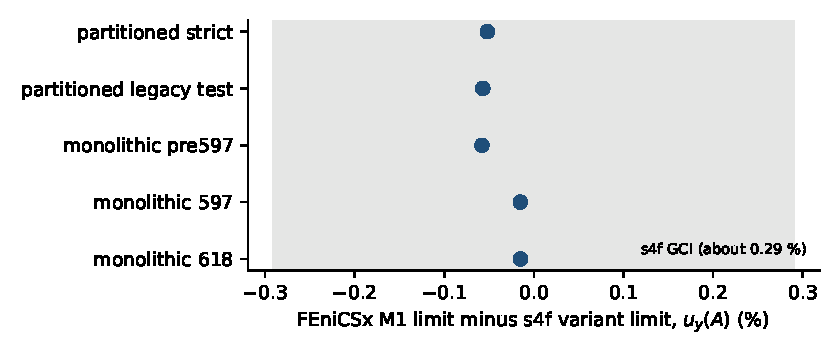
\includegraphics[width=0.7\textwidth]{paper-data/fenicsx_cavityflexiblebottom/figures/fenicsx_cavity_reference_variants}
\caption{$u_y(A)$: FEniCSx M1 limit minus each solids4foam variant limit, against the solids4foam GCI band (\legbc).}\label{fig:cv_variants}
\end{figure}
\paragraph{Other references: context only.}
Tukovi\'c~\citep{Tukovic2018} ($-0.25103$), ANSYS ($-0.25364$) and COMSOL ($-0.24306$, finest level; not monotone) differ from the FEniCSx limit by $4.4\,\%$, $5.4\,\%$ and $1.0\,\%$ in $u_y$ (\texttt{data/context\_comparison.csv}). No equivalence is claimed between any of them and the exact model: the paper records ANSYS and COMSOL as linear elastic with geometric nonlinearity (PRs~\#12, \#20, \#22; COMSOL equals StVK in intent, its plane strain or stress setting is not stated, and its load is about $0.7\,\%$ higher); the Tukovi\'c law is not confirmed. They are shown as context and attract no agreement or disagreement statement.

\section{A labelled sensitivity: current traction on reference area}\label{sec:cv_m2}
To size the effect of the interface measure, one level (L2, same mesh and $\Delta t$) was run with the plate loaded by $\bm\sigma_f\bm n_\mathrm{cur}$ per \emph{reference} area (a ``sensitivity measure''; the code calls it M2). The change relative to M1 is $|u_y|$ $+1.04\,\%$, $u_x$ $-1.9\,\%$, $F_y$ $5.4\times10^{-5}$ relative (smaller), left support reaction $-0.83\,\%$ (\texttt{data/m1\_vs\_labelled\_sensitivity.csv}).
\textbf{This is not the cavity tutorial's transfer.} Source reading of solids4foam commit 669d0f58d, per case (no solids4foam run tested it):
\begin{itemize}
\item \emph{cavityFlexibleBottom}: \texttt{solidModel nonLinearGeometryTotalLagrangianTotalDisplacement}; \texttt{nonLinGeomTotalLagTotalDispSolid.C} builds $\bm S_f=J\bm F^{-T}\bm S_{f,0}$, $|\bm S_f|$ and the traction on the current normal, and \texttt{enforceTractionBoundaries} (lines 251--384; non-high-order branch 371--380, \texttt{highOrderResidual} false by default and not set) applies $\text{force}=\text{traction}\times|\bm S_f|$ (also lines 480--500); \texttt{useUndeformedArea} defaults to false (\texttt{solidTractionFvPatchVectorField.C}, lines 43, 75--77) and is not set in \texttt{0/solid/D}.
\item \emph{blobInTreacle}: \texttt{solidModel linearGeometryTotalDisplacement}; \texttt{linGeomTotalDispSolid.C} (about lines 337--364) uses the reference normal and \texttt{mesh().magSf()}, i.e.\ traction $\times$ reference area (PR~\#69).
\end{itemize}
In both cases \texttt{fluidSolidInterface::updateForce()} hands over the fluid traction $\bm t=\bm\sigma_f\bm n_\mathrm{cur}$ per unit area (face to face). With Nanson's relation $\bm t\,\mathrm da=\bm\sigma_f\bm a\,\mathrm dS_0$, $\bm a=J\bm F^{-T}\bm N$, $\mathrm da=J_s\,\mathrm dS_0$ ($J_s=|\bm a|$): the total-Lagrangian path applies $\bm t\,J_s\,\mathrm dS_0=\bm t\,\mathrm da$, exact and equal to M1, whereas the linear-geometry path integrates the current-configuration traction over reference areas, $F_\mathrm{applied}=\int\bm t\,\mathrm dS_0$, which differs from the fluid-reported $\int\bm t\,\mathrm da$ by $\int(1-J_s)\bm t\,\mathrm dS_0$ (M2). The cavity path is therefore M1-equivalent in the area measure; the discretisations (finite volume against finite element) still differ.
The preregistered prediction (b) (M2 changes $|u_y|$ by $+0.3$ to $+1.2\,\%$ \emph{and moves it toward the reference}) rested on the premise that the tutorial is M2. It is \textbf{withdrawn as ill-posed}; its failure is kept: the size part holds ($+1.04\,\%$), the direction does not ($M1$ already sits $0.05\,\%$ from the strict partitioned limit \legbc and the sensitivity measure moves $1\,\%$ past it). The other preregistered predictions held ((a) L4 $u_y$ in $[-0.2380,-0.2407]$: $-0.24044$; (c) $F_y$ within $0.5\,\%$; (d) $|u_x|<1.1\times10^{-4}$).
The sensitivity run does \emph{not} satisfy the force-balance gate: the relative balance residual peaks at $1.3\times10^{-2}$ ($8.7\times10^{-3}$ at stop) against the gate of $10^{-8}$. This is expected by construction, because this measure is not force-conservative (plate load $\bm\sigma_f\bm n_\mathrm{cur}$, assembled fluid force $\bm\sigma_f\bm a$); it is not ``converged under the same gates''. The power identity still holds ($7\times10^{-13}$).

\section{What is claimed and what is not}\label{sec:cv_claims}
\begin{itemize}
\item \textbf{Claimed (exact model only).} A second implementation, by the same group and tooling lineage, of the cavityFlexibleBottom StVK plane-strain model, with accepted monotone sequences for $u_y(A)$ and $F_y$, a quantified pseudo-time, time-step and solver-tolerance error, a rigid-limit check, and a $u_y$ limit within $0.015$--$0.06\,\%$ and $F_y$ limit within $0.001$--$0.06\,\%$ of the solids4foam variants (inside their spread and GCI; \legbc).
\item \textbf{Not claimed.} Independence of a different group; second-order convergence of $u_y$ (order $\approx1.3$, pre-asymptotic) or a general order for $F_y$ (one accepted triple); equivalence of Tukovi\'c, ANSYS or COMSOL with the exact model; that the tutorial transfer is the sensitivity measure; that the consistency gates prove physical correctness; agreement below the solids4foam spread; effects of solids4foam PR~\#671 on any solids4foam value (reruns pending); a proved cause for the $u_y$ order (the corner hypothesis is neither confirmed nor rejected: the graded-mesh test failed); a resolution of the COMSOL difference.
\item \textbf{Limitations.} One mesh family; the sensitivity measure at one level; pseudo-time (not physical-time) solution; no external review; $\Delta x$--$\Delta t$ coupling and stabilisation inside the solids4foam sequences.
\item \textbf{Added value.} The solids4foam limit \legbc{} is shown to be reproduced by a numerically different discretisation of the same model (support that it is a property of the model rather than of one solver, which the plate-only check could argue only indirectly), and the transfer question for the cavity is addressed by source reading (no solids4foam run tested it) rather than by a labelled sensitivity.
\end{itemize}

\section*{AI-use disclosure (placeholder for author review)}
\hl{TBD by the authors:} AI coding and writing assistants (Anthropic Claude) were used to implement and run the FEniCSx code, post-process results, audit them internally and draft this text; the authors are to confirm, edit and take responsibility for the content, and to agree the wording against the journal's policy. No authorship is assigned to an AI system.

\bibliography{bibliography}

\end{document}
